\chapter{RC 7}
\recitation{7}{24 Nov. 18:30}{}

\section{Continuous Random Variables}

\subsection*{Joint p.d.f}
The concept for one variable r.v. still applies here. For continuous r.v., we won't use "probability at point". 
Instead, we will only use p.d.f in the context of \textbf{"measuring probability of event"}, i.e. \\
\cite{Und_Chatterjee}
Suppose that \(X_1, \dots, X_n\) are continuous r.v. defined on the same probability space. The n-tuple (means order things of length n) \(X = (X_1, \dots, X_n)\) is called a \textbf{random vector}. Note that 
\begin{itemize}
    \item \(X : \Omega \to  \mathbb{R}^n\)
    \item non-negative \(f: \mathbb{R}^n \to  \mathbb{R}\)  is the \textbf{joint p.d.f.} of \(X_1, \dots,X_n\) is such that for any "good" (i.e. measurable) set \(A \subseteq \mathbb{R}^n\), we measure the probability of \(X\in A\) by   
\[
    P(X \in A) = \int_A f(x_1, \dots, x_n)dx_1 \dots dx_n
\]

\begin{exercise}
    Given a joint p.d.f. \(f(x,y)\) defined by 
    \[
        f(x,y) = \begin{cases}
            1, &\text{ if } 0\leq x\leq 1, 0 \leq y \leq  1 ;\\
            0, &\text{ otherwise } .
        \end{cases}
    \]
    What is the probability of \(A = [\frac{1}{4}, \frac{1}{2}]\times [\frac{1}{3},\frac{2}{3}]\) 
\end{exercise}
    \item Independence \\
    As the concept in previous chapters on discrete r.v., independent for r.v.'s means that we can calculate the 
    probability of joint event "variable by variable", i.e. 
    \[
        P(X_{1} \in A_1, X_2 \in A_2 , \dots , X_n \in A_n ) = \prod_{i = 1}^n P(X_i \in A_{i} )
    \]
    The RHS equals (The p.d.f. of \(X_i\) is \(f_i(x_i)\)  )
    \[
      \int_{A_1} \cdots \int_{A_n} \prod_{i = 1}^n f_i(x_i) dx_1 \dots dx_n    
    \],
    and the LHS is 
    \[
        \int_{A_1 \times \cdots \times A_n  } f(x_1, \dots, x_n) dx_1 \dots dx_n    
    \]
    Hence, it is reasonable to define Independence by p.d.f., i.e. 
    \begin{remark}
       \(X_{1},\dots, X_n \)  are independent if 
       \[
            f(x_1, \dots, x_n) = \prod_{i=1}^n f_i(x_i)
       \]
    \end{remark} 
\end{itemize}      

\subsection{Multivariable change of variables}
Just remember what you learn in multivariable calculus, or implicit/explicit function theorem in advanced calculus. 
The intuition is: 
\begin{figure}[h]
    \centering
    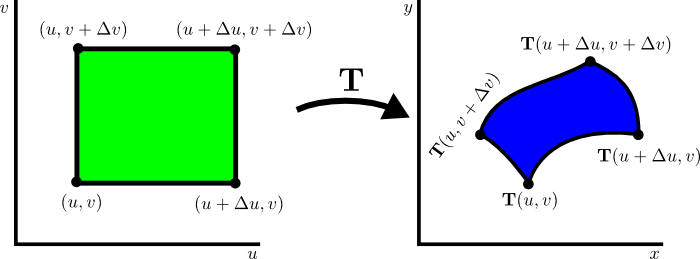
\includegraphics[width=0.8\textwidth]{./Figures/CoV.png}
    \caption{\label{fig:CoV_Jacobian}(TBD draw it yourself) Transformation \(T\) stretch the small rectangle, so we need to give a "different unit"  \(|\text{det}J_T|\) or \(\left|\frac{\partial (u,v)}{\partial (x,y)} \right|\) . \href{https://mathinsight.org/image/change_variable_area_transformation}{source}. }
\end{figure}

Usually you will be given transformation  \((x,y) = T(u,v) \). For example, if T is polar coordinate representation of (\(x,y\) ) and \((u,v) = (r,\theta )\). Then,  \(T(r,\theta ) = (r\cos(\theta ), r\sin(\theta ))\). 

Once acquiring \(T\), the area correction in \ref{fig:CoV_Jacobian} can be formally put down as
$$
dxdy = \left|\frac{\partial (x,y)}{\partial (u,v)} \right| dudv .
$$ 
Hence, the new p.d.f. \(g(v,w) \) is
\[
    g(u,v) = f(T(u,v)) \left| J_T \right|
\]  
\begin{exercise}
    Exercise 3,6,11
\end{exercise}

\section*{Extra}
\begin{itemize}
    \item Counterexample to Fubini theorem \\ 
    \[
        [f(i,j)]=\begin{bmatrix}1&0&0&0&\cdots
\\ -1&1&0&0&\cdots
\\0&-1&1&0&\cdots
\\0&0&-1&1&\cdots
\\\vdots&\vdots&0&-1&\cdots
\\\vdots&\vdots&\vdots&\vdots&\ddots
\\0&0&0&0&\cdots
\end{bmatrix}
    \] 
    \href{https://math.stackexchange.com/questions/3566631/counterexample-in-fubinis-theorem-non-integrable-function}{source}
\end{itemize}
hi